\documentclass[]{article}
\newcommand{\FileDepth}{../../..}
\usepackage[a4paper, total={15cm,23cm}]{geometry}
\usepackage[T1]{fontenc}
\usepackage{textcomp}%Not strictly necessary, but gives \textmu command for "micro."
\usepackage{fancyhdr}
\usepackage{amsmath}
\usepackage{amssymb}
\usepackage{graphicx}
\usepackage{xcolor}
\usepackage{tikz}
\usetikzlibrary{calc}
\usepackage{cancel}% Special for Activities 1 and 2.
%opening
\newcommand{\SecType}{R}
\newcommand{\Week}{8}
\title{PH 221 Week \Week}
\author{Benjamin Bauml}
\date{Summer 2024}
\pagestyle{fancy}
\rhead{PH 221}
\chead{Summer 2024}
\lhead{Week \Week}

% For Assignment, leave Purpose as 1. For Worksheet, set to 2. For Student Solution, set to 3. For Teacher Solution, set to 4.
% If you want keep the pieces from being called manually, set DefOnly to 0.
\newcommand{\Purpose}{1}
\newcommand{\DefOnly}{1}

% Version 2024-04-27
% Changes
% 2024-02-21 Added xstring package to enable smooth implementation of new \ModePage command.
% 2024-04-27 Set up to split activities and formatting aspects into separate files. Removed dependence on xcomment. Added an automatic counter to number the activities in a problem set.
% 2024-05-19 Revised old format for \TeachingTips command, which did not support \DefOnly.
\usepackage{tcolorbox}
\usepackage{xstring}
% You will want the following four lines in your document (the last two uncommented):
% For Assignment, leave Purpose as 1. For Worksheet, set to 2. For Student Solution, set to 3. For Teacher Solution, set to 4.
% If you want keep the pieces from being called manually, set DefOnly to 0.
%\newcommand{\Purpose}{4}
%\newcommand{\DefOnly}{1}
\newcommand{\Exclusion}{0}
\newcommand{\PageTurn}{0}
\newcommand{\GrayProb}{0}
\newcommand{\Tipsy}{0}

% Assignment
\if\Purpose1
\renewcommand{\Exclusion}{1}
\fi
% Worksheet
\if\Purpose2
\renewcommand{\Exclusion}{1}
\renewcommand{\PageTurn}{1}
\fi
% Student Solution
\if\Purpose3
\renewcommand{\PageTurn}{1}
\renewcommand{\GrayProb}{1}
\fi
% Teaching Copy
\if\Purpose4
\renewcommand{\PageTurn}{1}
\renewcommand{\GrayProb}{1}
\renewcommand{\Tipsy}{1}
\fi

\def \NewQ {0}
\def \PForce {0}
\newcommand{\MaybePage}[1]{
	\def \PForce {#1}
	\if\PForce1
	\newpage
	\else
	\if\NewQ0
	\gdef \NewQ {\PageTurn}
	\else
	\newpage
	\fi
	\fi
}

\newcommand{\ModePage}[1]{
	\IfSubStr{#1}{\Purpose}{\newpage}{}
}

\newcounter{ActNumber}
\setcounter{ActNumber}{0}

\newcommand{\Problem}[4][0]{%The first argument is optional, and if it is set to 1, the \newpage will be forced. The second argument is the name of the activity, the third is the command the activity is stored as, and the fourth is the actual problem statement.
\newcommand{#3}{
\MaybePage{#1}
\addtocounter{ActNumber}{1}
\section*{\SecType\Week-\theActNumber: #2}
\if\GrayProb1
\begin{tcolorbox}[colback=lightgray,colframe=lightgray,sharp corners,boxsep=1pt,left=0pt,right=0pt,top=0pt,bottom=0pt,after skip=2pt]
\else
\begin{tcolorbox}[colback=white,colframe=white,sharp corners,boxsep=1pt,left=0pt,right=0pt,top=0pt,bottom=0pt,after skip=2pt]
\fi
#4
\end{tcolorbox}\noindent
}
\if\DefOnly0
\else
#3
\fi
}
	
\newcommand{\ProblemSub}[3][0]{%The first argument is optional, and if a string of numbers is entered into it, it will force a \newpage in any \Purpose that shows up in the string. For example, "13" would lead to the newpage being forced in modes 1 and 3. The second is the command the activity is stored as, and the third is the actual problem statement.
\newcommand{#2}{
\ModePage{#1}
\if\GrayProb1
\begin{tcolorbox}[colback=lightgray,colframe=lightgray,sharp corners,boxsep=1pt,left=0pt,right=0pt,top=0pt,bottom=0pt,after skip=2pt]
\else
\begin{tcolorbox}[colback=white,colframe=white,sharp corners,boxsep=1pt,left=0pt,right=0pt,top=0pt,bottom=0pt,after skip=2pt]
\fi
#3
\end{tcolorbox}\noindent
}
\if\DefOnly0
\else
#2
\fi
}
		
\newcommand{\Solution}[2]{%The first argument is the command the solution is stored as, and the second is the actual solution.
\newcommand{#1}{
\if\Exclusion0
#2
\fi
}
\if\DefOnly0
\else
#1
\fi
}
		
\newcommand{\ProblemFig}[2]{%The first argument is the command the figure is stored as, and the second is the actual figure.
\newcommand{#1}{
\begin{figure}[h]
#2
\end{figure}
}
\if\DefOnly0
\else
#1
\fi
}

\newcommand{\TeachingTips}[2]{%The first argument is the command the tip is stored as, and the second is the actual tip.
\newcommand{#1}{
\if\Tipsy1
\begin{tcolorbox}[colback=lightgray,colframe=black]
#2
\end{tcolorbox}
\fi
}
\if\DefOnly0
\else
#1
\fi
}

%\newcommand{\FBDaxes}[3]{
	\begin{scope}[shift={(#1)},rotate=#2]
		% x-axis
		\draw[thick,->] (-2,0) -- (2,0);
		\node[anchor=west] at (2,0) {$x$};
		% y-axis
		\draw[thick,->] (0,-2) -- (0,2);
		\node[anchor=west] at (0,2) {$y$};
		\coordinate (#3) at (0,0);
	\end{scope}
}
\newcommand{\FBDvectorMA}[4]{
	\begin{scope}[shift={(#1)}]
		\coordinate (#4tip) at ({#2*cos(#3)},{#2*sin(#3)});
		\draw[ultra thick,blue,->] (#1) -- (#4tip);
	\end{scope}
}
\newcommand{\FBDvectorXY}[3]{
	\begin{scope}[shift={(#1)}]
		\coordinate (#3tip) at (#2);
		\draw[ultra thick,blue,->] (0,0) -- (#3tip);
	\end{scope}
}
\newcommand{\FBDdot}[1]{
	\filldraw[black] (#1) circle (3pt);
}% May want this to eventually replace the borrowed images.

\begin{document}
\maketitle
\begin{center}
	This material is borrowed/adapted from Chapter 11 of the \textit{Student Workbook} for \textit{Physics for Scientists and Engineers}.
\end{center}

\Problem{Comparing Pushed Particles}{\ComPushP}{
Particle A has less mass than particle B. Both are pushed forward across a frictionless surface by equal forces for 1 s. Both start from rest.
}
\ProblemSub{\ComPushPA}{
(a) Compare the amount of work done on each particle. That is, is the work done on A greater than, less than, or equal to the work done on B? Explain.
}
\Solution{\ComPushPASol}{

The amount of work done by a force depends on the sizes of the force and the displacement of the object under that force. The same force is applied to both particles, but since A has less mass, it will accelerate more and have greater displacement. Therefore, the work done on A is greater.
}
\ProblemSub{\ComPushPB}{
(b) Compare the impulses delivered to particles A and B. Explain.
}
\Solution{\ComPushPBSol}{

Because the same net force is applied over the same elapsed time, the impulses are the same.
}
\ProblemSub{\ComPushPC}{
(c) Compare the final speeds of particles A and B. Explain.
}
\Solution{\ComPushPCSol}{

Let the particles move along the $ x $-axis so we may discuss the components of their momenta. The same impulse $ J_{x} $ is delivered to both particles, and since they both start from rest, we know $ p_{ix} = 0 $. This gives
\[
J_{x} = \Delta p_{x} = p_{fx} - \cancel{p_{ix}} = p_{fx}.
\]
As such, both particles have the same final momentum:
\[
p_{fx} = m_{A}v_{fA} = m_{B}v_{fB}.
\]
However, since $ m_{A} < m_{B} $, we must conclude that $ v_{fA} > v_{fB} $.
}
\newcommand{\Arxr}{\text{archer}}
\newcommand{\Arrw}{\text{arrow}}
\Problem{Ice Archer and Cadillac Crash}{\IceCad}{
For this activity, we will be looking at two situations that mirror each other: a superelastic collision and a perfectly inelastic collision. We want to see how these situations are alike and how they are different.
}
\ProblemSub{\IceCadA}{
(a) For each situations below, prepare a pictorial representation.
\begin{itemize}
	\item Draw pictures of ``before'' and ``after.''
	\item Define symbols relevant to the problem.
	\item List known information, and identify the desired unknown.
\end{itemize}
}
\ProblemSub{\IceCadI}{
	
(i) A 50 kg archer, standing on frictionless ice, shoots a 100 g arrow at a speed of 100 m/s. What is the recoil speed of the archer?
}
\Solution{\IceCadAISol}{

\begin{figure}[h]
	\centering
	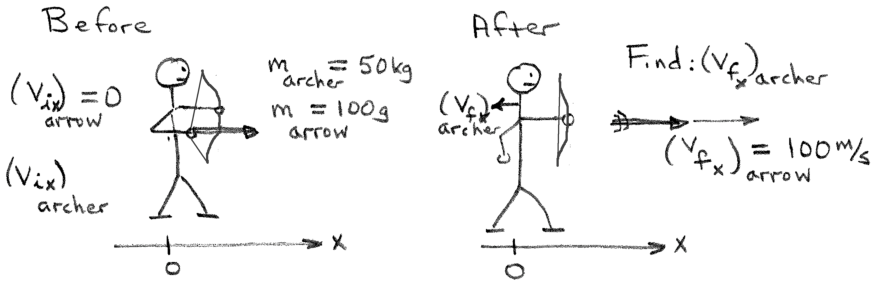
\includegraphics[scale=0.7]{\FileDepth/Activities/Ice_Archer_and_Cadillac_Crash/Archer_on_Ice.pdf}
\end{figure}
}
\ProblemSub{\IceCadII}{
	
(ii) The parking brake on a 2000 kg Cadillac has failed, and it is rolling slowly, at 1 mph, toward a group of small, innocent children. As you see the situation, you realize there is just time for you to drive your 1000 kg Volkswagen head-on into the Cadillac and thus save the children. With what speed should you impact the Cadillac to bring it to a halt?
}
\Solution{\IceCadAIISol}{

\begin{figure}[h]
	\centering
	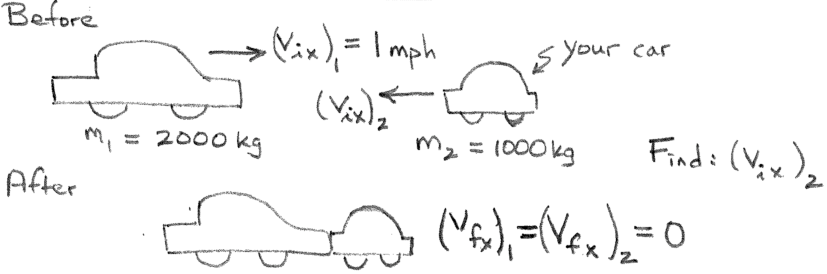
\includegraphics[scale=0.7]{\FileDepth/Activities/Ice_Archer_and_Cadillac_Crash/Cadillac_Collision.pdf}
\end{figure}
}
\ProblemSub[34]{\IceCadB}{
(b) For both of these situations, we want to apply conservation of momentum, but the details of why we can do this are slightly different. How can we justify conservation of momentum for the following systems?
}
\ProblemSub{\IceCadBI}{
(i) The archer and the arrow.
}
\Solution{\IceCadBISol}{

There is no friction, and the normal force from the ice on the combined arrow and archer system cancels with the force of gravity on the system. As such, there will be no net force on the system, and therefore no impulse. Without impulse, momentum is conserved.

We have to look at the whole system, because the normal force on the archer from the ice does not balance with just the force of gravity on the archer; the archer is also supporting the weight of the arrow. By defining the system to be both the archer and the arrow, the internal forces between the two---friction, normal force, and tension---do not affect the net external force on the system as a whole.

Even if there were a net external force---say the archer was standing in an elevator with a frictionless floor accelerating upward---we might still be able to assume the impulse is negligible, as the arrow leaves the bow very quickly, and impulse is smaller if the time of the interaction is smaller.
}
\ProblemSub{\IceCadBII}{
(ii) The Cadillac and the Volkswagen.
}
\Solution{\IceCadBIISol}{

The normal forces on the cars are balanced against the forces of gravity, so the vertical direction has no net force, but tires are built for traction, so friction cannot be ignored. However, crashes are usually quite quick events, and the forces between crashing objects are usually quite large. As such, the impulse can be assumed to be negligible, both due to the interaction being brief, and because the external forces are likely far less significant in magnitude when compared to the internal ones.
}
\ProblemSub{\IceCadC}{
(c) Solve the two situations for the desired quantity. Make sure to solve symbolically before plugging in numbers.
}
\ProblemSub{\IceCadCI}{
(i) What is the recoil speed of the archer?
}
\Solution{\IceCadCISol}{

The combined initial momentum of the archer and arrow (which is zero, since they both start from rest) is equal to the combined final momentum of the pair:
\[
\begin{split}
	m_{archer}\cancel{(v_{ix})}_{\Arxr} + m_{\Arrw}\cancel{(v_{ix})}_{\Arrw} & = m_{\Arxr}(v_{fx})_{\Arxr} + m_{\Arrw}(v_{fx})_{\Arrw} \\
	0 & = m_{\Arxr}(v_{fx})_{\Arxr} + m_{\Arrw}(v_{fx})_{\Arrw} \\
	(v_{fx})_{\Arxr} & = -\frac{m_{\Arrw}}{m_{\Arxr}}(v_{fx})_{\Arrw} \\
	& = -\frac{0.1\text{ kg}}{50\text{ kg}}(100\text{ m/s}) \\
	& = - 0.2\text{ m/s}.
\end{split}
\]
The archer's recoil speed is 0.2 m/s.
}
\ProblemSub{\IceCadCII}{
(ii) With what speed should you impact the Cadillac to bring it to a halt?
}
\Solution{\IceCadCIISol}{

The combined initial momentum of the Cadillac and Volkswagen is equal to the combined final momentum of the pair (which is zero, since they crash to a dead stop):
\[
\begin{split}
	m_{1}(v_{ix})_{1} + m_{2}(v_{ix})_{2} & = m_{1}\cancel{(v_{fx})}_{1} + m_{2}\cancel{(v_{fx})}_{1} \\
	m_{1}(v_{ix})_{1} + m_{2}(v_{ix})_{2} & = 0 \\
	(v_{ix})_{2} & = -\frac{m_{1}}{m_{2}}(v_{ix})_{1} \\
	& = -\frac{2000\text{ kg}}{1000\text{ kg}}(1\text{ mph}) \\
	& = - 2\text{ mph}.
\end{split}
\]
You must hit the Cadillac at 2 mph to stop it.
}
\ProblemSub{\IceCadD}{
(d) Identify and check special cases for each of these situations. If you examine a particular special case for one situation, adjust it to apply to the other situation. The math will be practically identical, but the physical interpretation will be distinct.
}
\Solution{\IceCadDSol}{

\noindent\textbf{\underline{Case 1: Equal Masses}}

For both situations, we can think about the internal forces. The internal forces between the two objects are equal and opposite (as they are a 3rd law pair), and equal forces on equal masses result in equal accelerations. Both forces act for the duration of the interaction, and the same acceleration over the same time means the same change in speed.

If $m_{\Arxr}=m_{\Arrw}$ (the archer is firing an arrow with the mass of an equally large human), then $(v_{fx})_{\Arxr} = -(v_{fx})_{\Arrw} = -100$ m/s. Since both start from rest, they end up with the same speed due to the internal interactions.

If $m_{1}=m_{2}$ (the Cadillac and the Volkswagen have the same mass), then $(v_{ix})_{2} = -(v_{ix})_{1} = -1$ mph. They have to start with the same speed for the internal interactions to bring them both to a stop.

\noindent\textbf{\underline{Case 2: Archer/Volkswagen Far More Massive}}

If $m_{\Arrw} \ll m_{\Arxr}$ (the archer is firing an arrow with negligible mass), then $(v_{fx})_{\Arxr} \approx 0$ m/s. The archer does not recoil significantly when propelling something with far less mass---analogously, if you flick a small beetle off of your arm, you will not feel a significant kick back from that interaction.

If $m_{1} \ll m_{2}$ (the Cadillac is of negligible mass in comparison to the Volkswagen), then $(v_{ix})_{2} \approx 0$ mph. The Volkswagen is so massive that its velocity won't change when it strikes the Cadillac, and so it must be stopped at the time of the collision for both vehicles to be still afterward.

\noindent\textbf{\underline{Case 3: Arrow/Cadillac Far More Massive}}

If $m_{\Arrw}\gg m_{\Arxr}$ (the archer is firing an arrow far more massive than a person), then $(v_{fx})_{\Arxr} \approx \infty$. If you try to propel an extremely massive object, it will barely budge, and you will be propelled backward. In this situation, the archer successfully made the massive arrow do more than budge (they made it go 100 m/s to be exact), so they were sent absolutely flying in the opposite direction to make that happen.

If $m_{1}\gg m_{2}$ (the Cadillac has far more mass than the Volkswagen), then $(v_{ix})_{2} \approx \infty$. To stop a massive object quickly requires a large amount of force---its vast inertia must be overcome to get any significant acceleration. Similarly, to stop a fast moving object quickly also requires a large amount of force---the large change in velocity requires a commensurately large acceleration. To make a massive object and a small object stop each other, the small object needs a correspondingly large speed to have comparable momentum. The great internal forces of the collision will bring both to a stop.
}
\end{document}